Firstly, we evaluate the fidelities achieved by the different protocols as a function of the number of QAOA layers (Fig.~\ref{fig:fidelity_layers}). Three distinct trends are observed:  
\begin{itemize}
    \item For $N = 25$, the \texttt{standard} protocol performs better at shallow depths, but both \texttt{linear} protocols eventually surpass it.  
    \item For $N = 77$, both \texttt{linear} protocols consistently outperform the \texttt{standard} protocol across all layers.  
    \item For $N = 143$, the \texttt{standard} protocol initially leads, until a sudden fidelity jump in one of the \texttt{linear} protocols overtakes it.  
\end{itemize}

As the problem size increases, the third behavior---a sudden jump in fidelity---appears more frequently. The underlying reasons for this phenomenon will be analyzed in Chapter~\ref{Chapter:Discussion}.  

\begin{figure}[h]
    \centering
    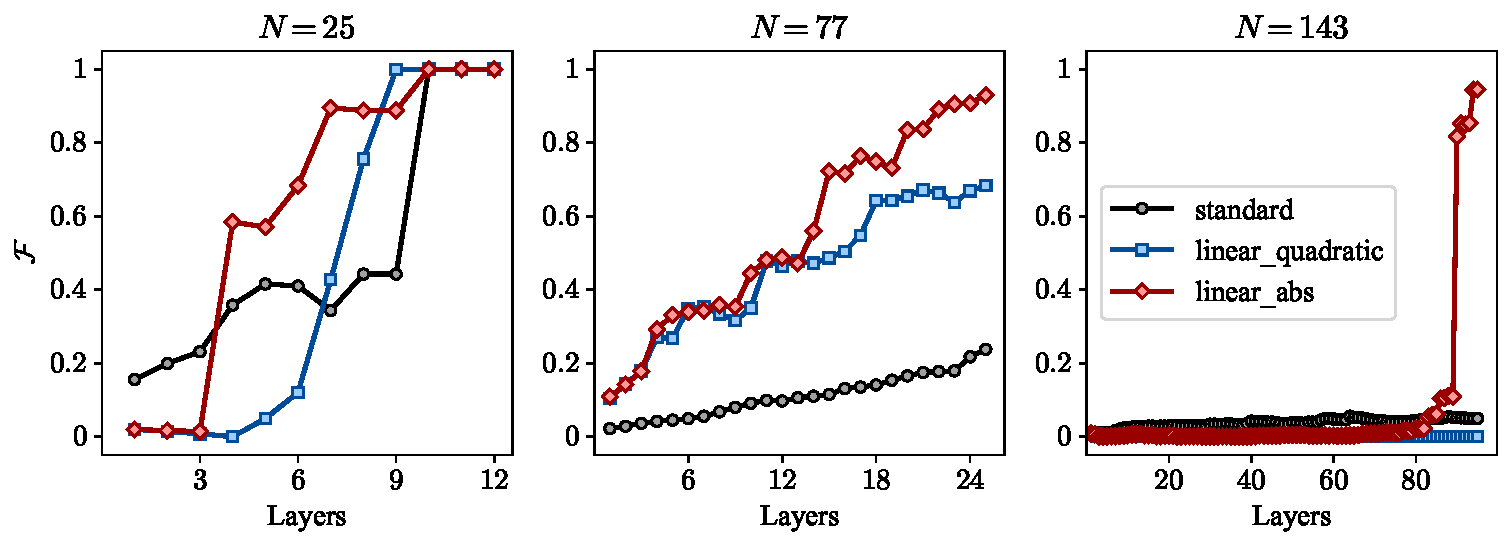
\includegraphics[width=1\textwidth]{04-results/figs/fidelity_layers_2577143.pdf}
    \caption{Fidelity versus QAOA layer depth. Larger problems require deeper circuits to achieve significant fidelities.}
    \label{fig:fidelity_layers}
\end{figure}

To complement the fidelity analysis, Fig.~\ref{fig:populations} depicts the state populations
at the end of each protocol, with valid solutions highlighted by dark-colored bars.

\begin{figure}[h]
    \centering
    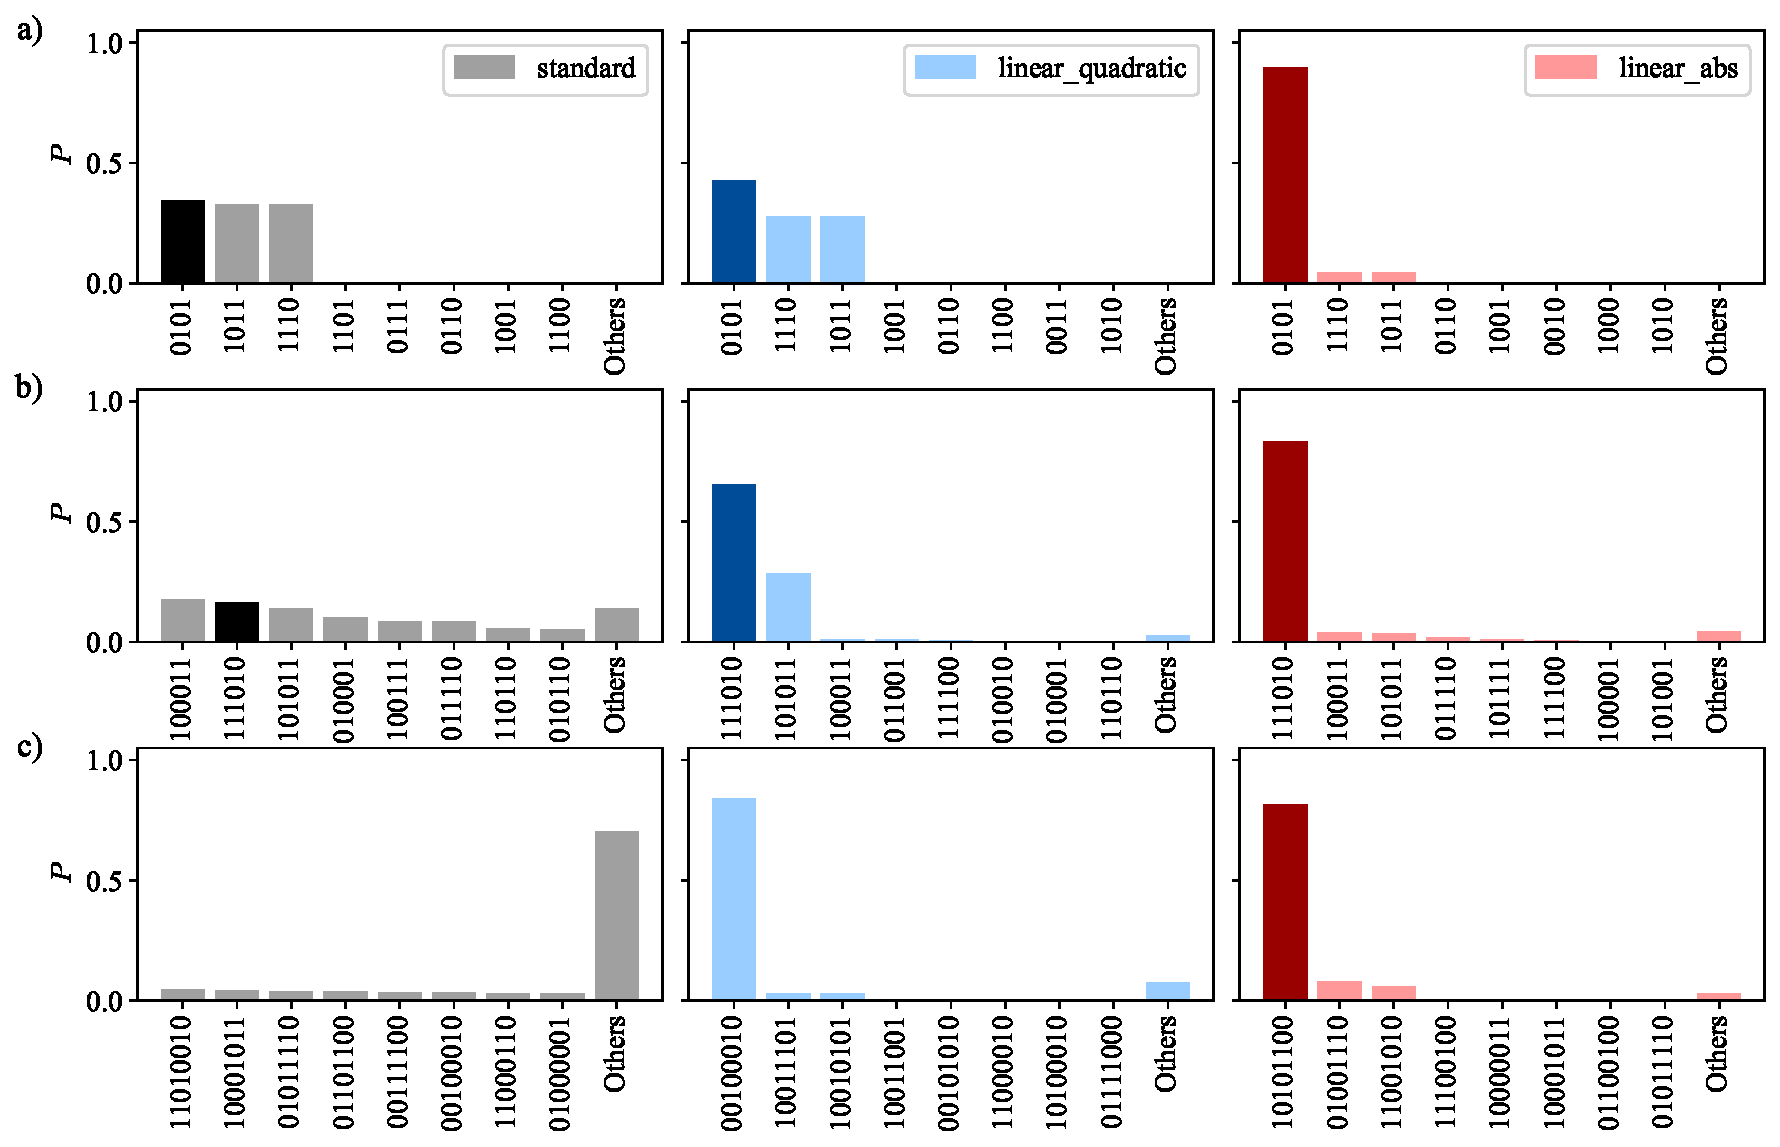
\includegraphics[width=0.8\textwidth]{04-results/figs/populations_2577143.pdf}
    \caption{Final state populations for (a) $N=25$, (b) $N=77$, and (c) $N=143$. The number
    of layers was fixed as the minimum required to reach at least 80\% fidelity by any
    protocol. Solution states are shown as dark-colored bars.}
    \label{fig:populations}
\end{figure}

Although fidelity as a function of depth already demonstrates the improved performance of the \texttt{linear} protocols, it is essential to evaluate them in terms of quantum resources. Specifically, we compare protocols using the number of two-qubit gates as the resource metric (Fig.~\ref{fig:fidelity_gates}). In these terms, the advantage of the \texttt{linear} protocols becomes clearer: they achieve significantly higher fidelities while requiring far fewer quantum operations.  

\begin{figure}[h]
    \centering
    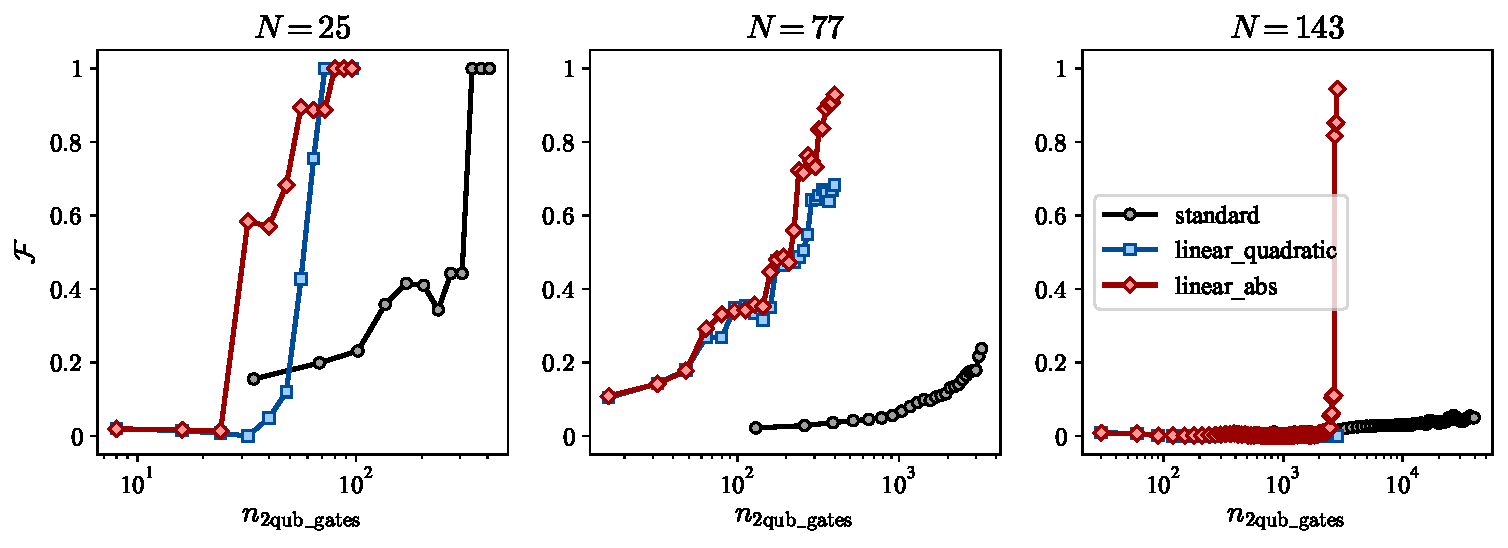
\includegraphics[width=1\textwidth]{04-results/figs/fidelity_gates_2577143.pdf}
    \caption{Fidelity versus the number of two-qubit gates. This metric highlights the resource efficiency of the \texttt{linear} protocols.}
    \label{fig:fidelity_gates}
\end{figure}

Finally, as a summarizing plot, Fig.~\ref{fig:accumulated_probability} presents a metric that
enables a consistent comparison between protocols across problem sizes. For larger problem instances,
fidelity does not always reach the same reference level within practical resource limits,
which makes direct fidelity thresholds less suitable as a single benchmark. To address this,
we consider how each protocol concentrates probability within the most relevant portion of
the spectrum, providing a way to compare performance across different problem sizes.

\begin{figure}[h]
    \centering
    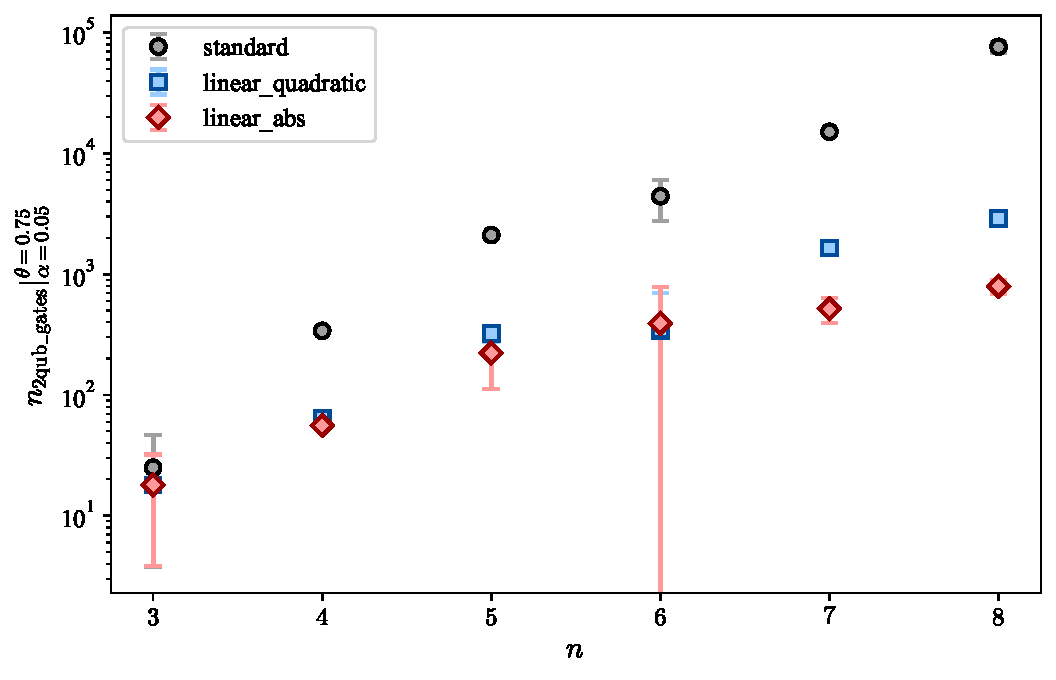
\includegraphics[width=0.75\textwidth]{04-results/figs/accumulated_probability.pdf}
    \caption{Number of two-qubit gates required to accumulate at least 75\% of the total probability
    within the 5\% of eigenstates closest to the solution, aggregated by problem size (number of qubits).
    Error bars represent variability across different instances with the same size.}
    \label{fig:accumulated_probability}
\end{figure}